\section{Experimental Results}
\label{sec:experimental_results}
%In the following section summarizes the results from experiments with the soft manipulator. 
We now discuss the grasping of objects as well as the repeatability and success rate of the autonomous system.
 
\subsection{Experimental Platform}
The \dr{soft manipulation} system we developed for this work is shown in Figure~\ref{fig:experimental_platform}.
%The planar six segment soft rubber manipulator consists of twelve distributed elastomer actuators. This manipulator moves with minimal friction on a level plane.
%A soft rubber gripper is fixed to the tip of the manipulator.
Each arm segment is 6.27\unit{cm} and the soft gripper is 10.6\unit{cm} long.
The localization system OptiTrack Flex 3 by Natural Point provides real-time measurements of marked points both along the inextensible back of the manipulator and on top of the object. 
A rigid frame holds all the subsystems \rkk{as a mobile presentation platform} together providing reliable hardware experiments without the need for recalibration.

\begin{figure}[htbp]
\begin{centering}
  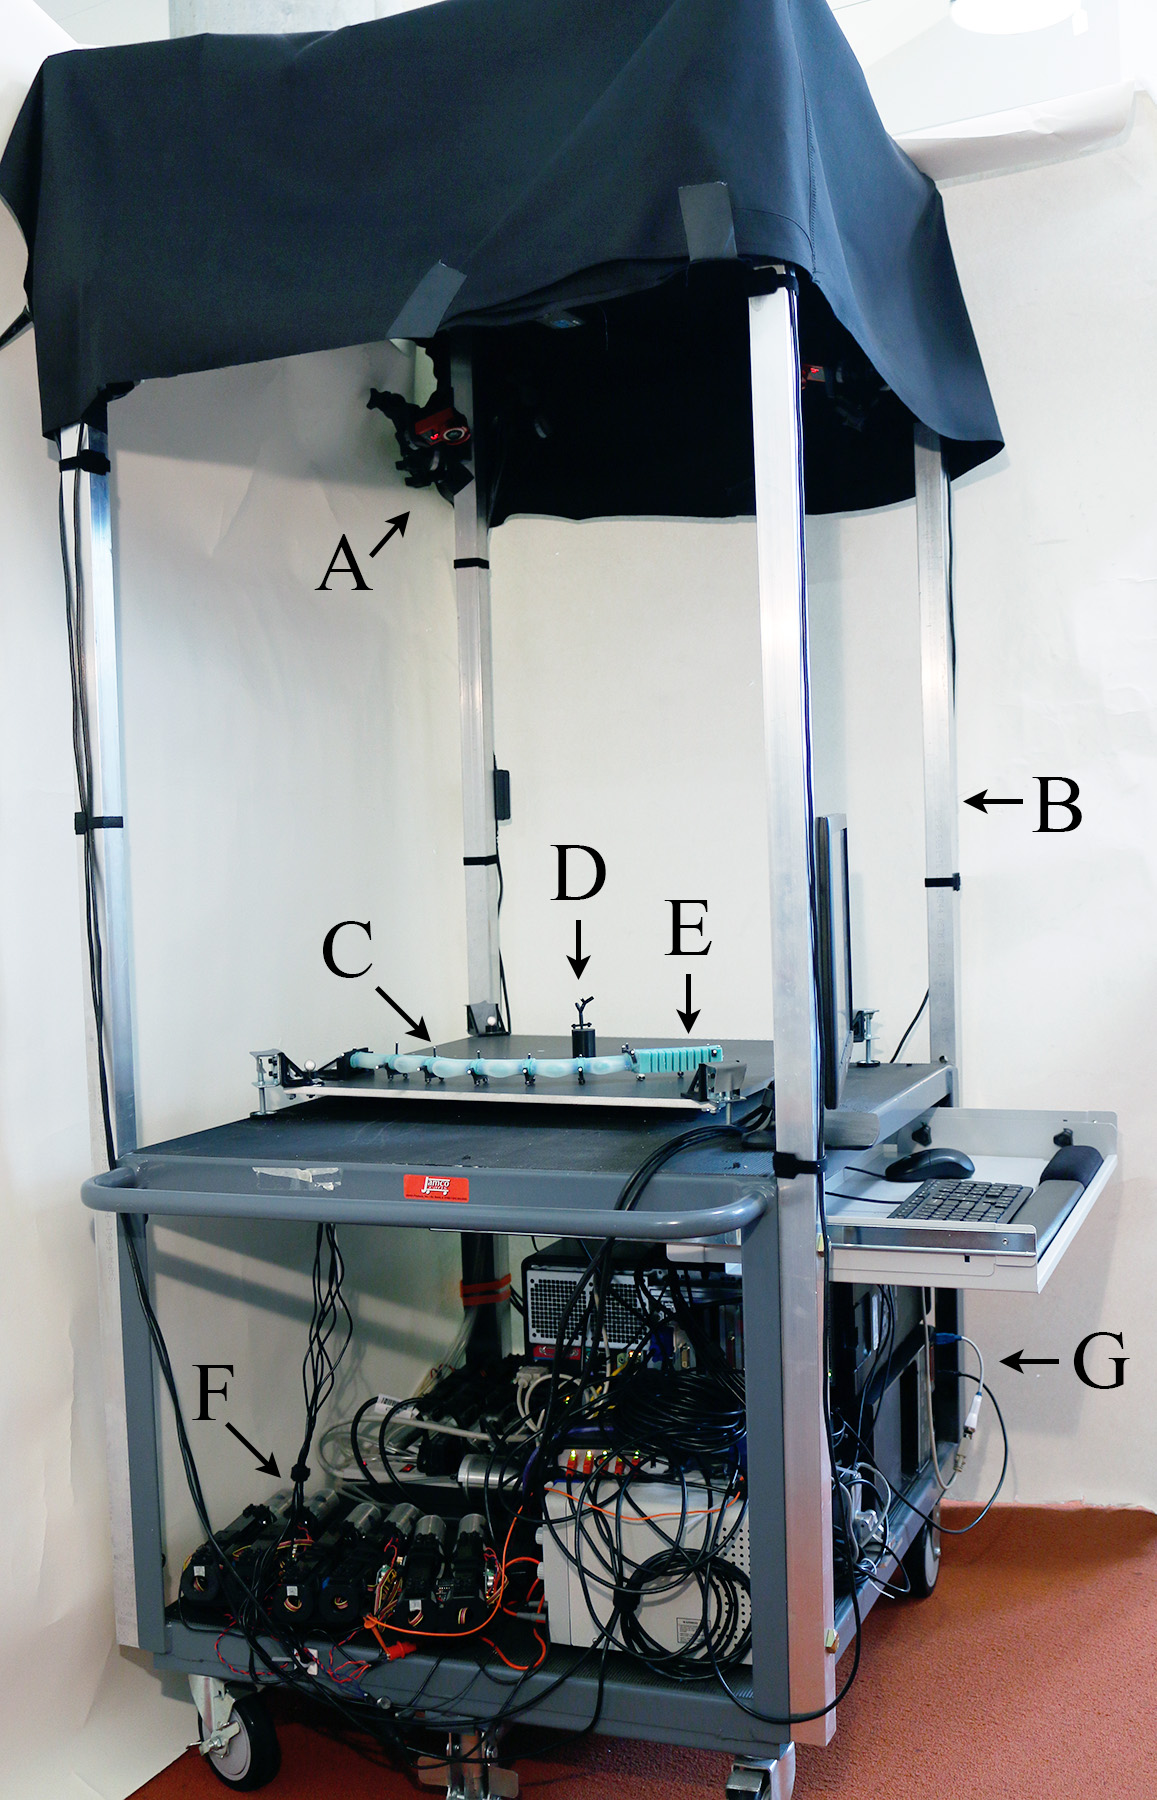
\includegraphics[width=2.0in]{Figures/system_overview/sys_overview_smaller}\\
  \caption{System Overview. The system is composed of (\textbf{A}) a motion capture system, (\textbf{B}) rigid frame, (\textbf{C}) soft six segment planar manipulator, (\textbf{D}) an object within the grasp envelope, (\textbf{E}) a soft gripper fixed to the manipulator, (\textbf{F}) a fluidic drive cylinder array to control actuation, and (\textbf{G}) computers for real-time processing and control.} \label{fig:experimental_platform}
\end{centering}
\end{figure}


%\subsection{Grasping Delicate Objects}
%\rkk{It was shown in \cite{marchese2015recipe} that pleated grippers of similar dimensions like the one used in this work can be contiuously actuated in a pressure range of 0-60\unit{kPa} and create blocking forces in the range of 0-2\unit{N}. This fine actuation range and the fact that soft manipulators easily conform to shapes implies that grasping delicate objects should be possible.}
%The manipulator in fact picks up delicate objects \rkk{such as eggs, shuttlecocks or bakery items} without \rkk{squishing} or breaking those. 
%Figure~\ref{fig:egg_approach_sequence} shows \rkk{for example} how the manipulator approaches and grasps an egg.
%Delicate objects can be manipulated without requiring a shape or a force sensor within its structure, since the compliant gripper body conforms to the object.
%Rigid-bodied grippers usually rely on force sensing or another type of sensory feedback to avoid damage caused to the object.

\begin{figure}[htb]
\centering
   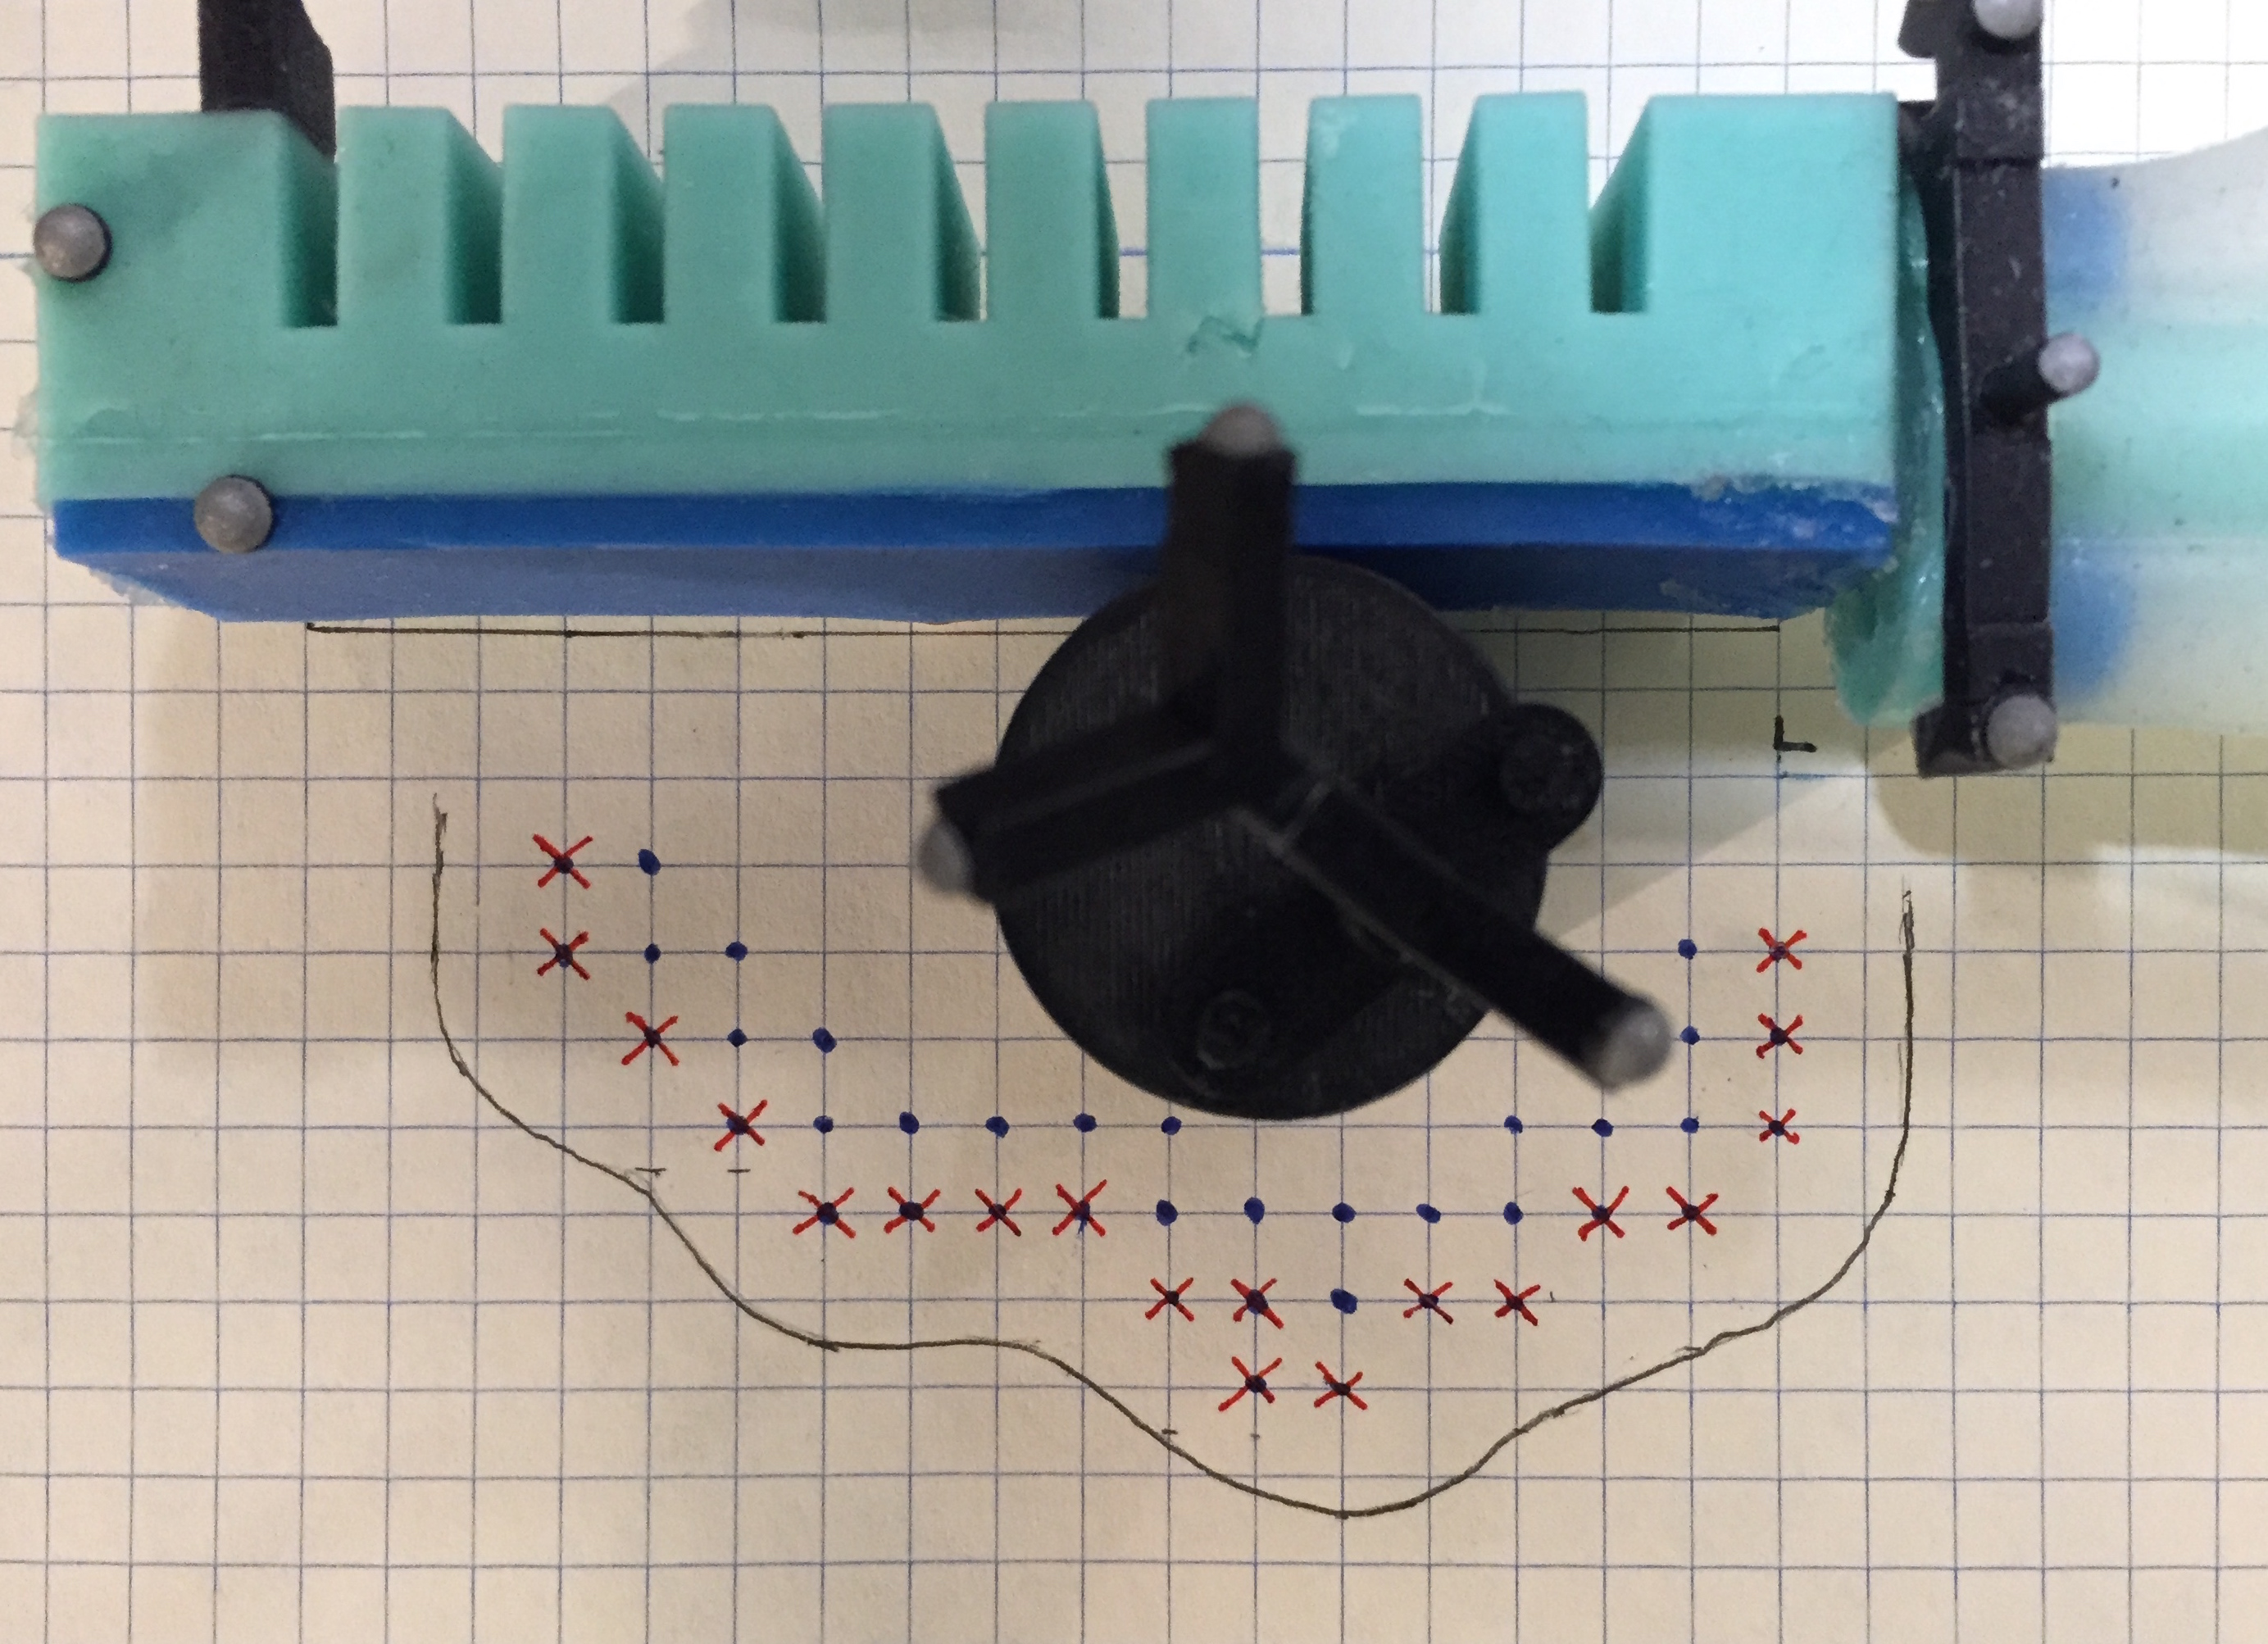
\includegraphics[width=0.8\columnwidth]{Figures/experimental_results/uncertainty}
   \caption{Experimental characterization of the gripper's capture region: the allowable positioning uncertainty is determined through repeated placements of the center of a cylindrical object at different points on a 5\unit{mm} grid relative to the gripper. Blue dots indicate all object center positions for which a grasp could be performed successfully, red crosses show the positions where a grasp failed. The grey line outlines an area for the object to be positioned within so the gripper can grasp it. The evaluation of the capture region was performed similarly to a method described in \cite{dogar2010push}.}
   \label{fig:grasp_uncertainty}
\end{figure} 

\subsection{Grasp Experiments}
\rkk{Using the experimental platform in Figure~\ref{fig:experimental_platform}, we implemented the planning algorithm described in Section~\ref{sec:processing_and_control}.
We evaluated the manipulator system for repeatability and ability to handle uncertainty.
The experiments consisted of picking and placing several objects of unknown geometry placed at an unknown location.
We measured the execution time and captured the location data during the experiments.
Specifically,}
we performed over 200 experimental grasp-and-place trials at randomly chosen positions within the reachable workspace to demonstrate the capabilities and repeatability of our system.
We successfully picked up various objects such as eggs, shuttlecocks, bakery items, cups, light bulbs, and tape holders. 
The objects had an enclosing diameter in the range of 2-5\unit{cm}. 
The results of a subset of those experimental trials are shown in Figure~\ref{fig:allTestsOverlaid}.
One representative approach, grasp, and retract move is shown in Figure~\ref{fig:oneTrialVsTime}.
In 23 of 25 experimental trials shown, the manipulator successfully achieved the task of grasping an object and placing it at a bin location shown in red.
\rkk{The test object has a weight of 18\unit{g} and a diameter of 3.3\unit{cm}.}
The object was placed five times on each of the five points marked on the board.
The markers only serve as a reference point for the user to place the object roughly at the same point at every repetition.
The user's placing accuracy is not important to the algorithm, \rkk{since the tracking system re-registers the position of the object every time it is placed.}
The five points were chosen to approximately represent the major portion of the manipulator's reachable workspace.
As long as the root of the gripper stops so that the object is located within the capture region, the gripper will pick it up through its sweeping closing motion. The capture region is outlined in grey in Figure~\ref{fig:grasp_uncertainty}. 

The evaluation of the capture region is performed similarly to a method described in Dogar and Srinivasa\cite{dogar2010push} work on determining capture regions for a push-grasp of a classical robotic gripper.
\rkk{Grid paper and fine markings on all four sides of the round object ensure that the placement by the user is accurate within $\pm$1\unit{mm} in relation to the discrete placement locations on the grid. This test serves as a qualitative measure to show qualitatively a relation between object size to gripper size to area of successful grasp.}
\rkk{This characterization was repeated two times, resulting in nearly identical capture regions.}
Despite positioning inaccuracies of the soft manipulator, the gripper can nevertheless successfully perform a grasp of an object. 
\rkk{The successful capture region can be characterized by about half a gripper length in diameter.}

When the arm reaches \rkk{its straight pose within a relatively large delta}, it drops the object.
\rkk{For these experiments, we focus on showing the capability of picking up objects at various places and moving them around, there is no emphasis set on having to drop off the object at a specific place. To indicate that the arm can move the object after grasping, the arm was controlled to go back to the fully straight pose. When the arm reached the final straight pose within a 1\unit{cm} delta, the gripper was set to release and drop the object. It was not ensured by the planner that the arm had to first settle to zero velocity at the final straight pose. As a consequence of this, the experimental data indicates as a red bin a relatively wide drop off area.}

\begin{figure*}[htbp]
\begin{centering}
  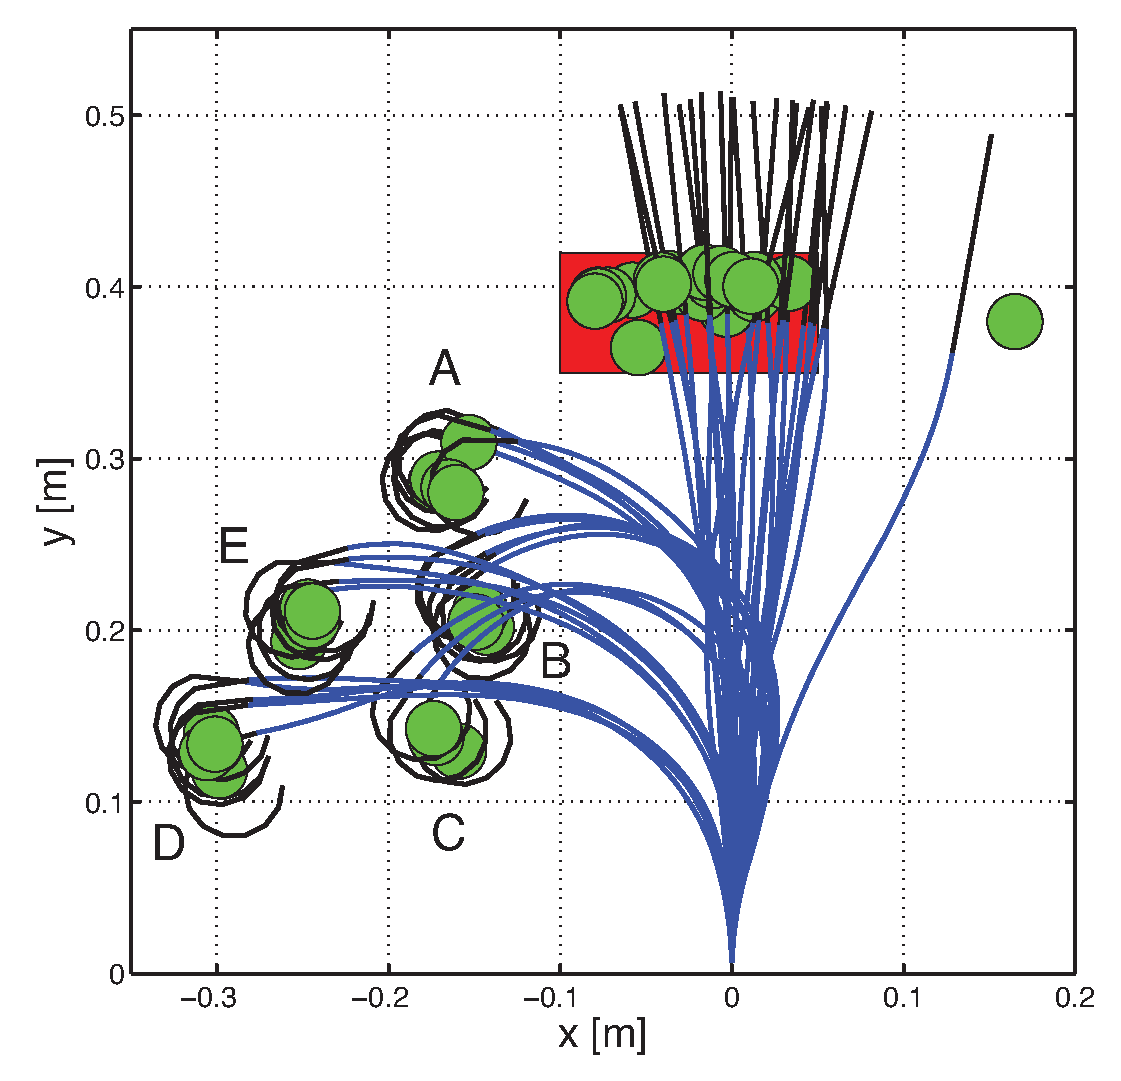
\includegraphics[width=0.5\textwidth]{Figures/experimental_results/allTestsOverlaid.eps}
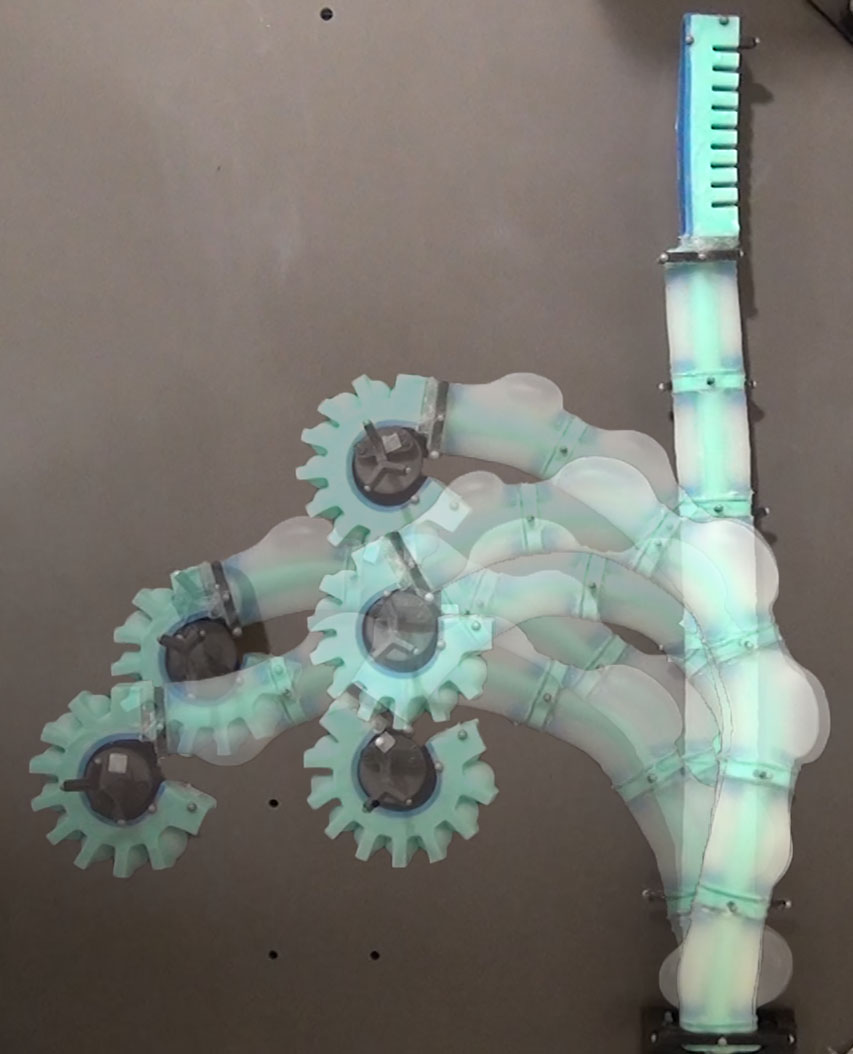
\includegraphics[width=0.385\textwidth]{figures/experimental_results/five_grasps.jpg}
\caption[Left: All 25 experimental grasping trials.]{Left: Complete set of experimental grasp-and-place trials. In these experiments, the arm moves from an initial straightened configuration to grasp a round object placed in one of five locations (A-E). The arm then returns the object to a bin location shown in red. For each trial, a seven degrees of freedom manipulator representation is generated at both the \emph{grasped} and \emph{released} state using experimental data and is shown in blue. The corresponding 1 DOF end-effector representation is shown in black. The round object's measured position at each state is shown in green. In one of the trials, the grasp and return was successfully performed, but an overshoot over the final bin location caused the gripper to drop off the small table it is moving on. Right: Overlaid photographs of the manipulator grasping an object placed at each of the five locations. }\label{fig:allTestsOverlaid}
\end{centering}
\end{figure*}

The unsuccessful trials happened due to stick-slip friction between the roller bearings and the table surface.
Our kinematic modeling does not account for this non-linear behavior, which acts as a disturbance and can lead to failure to arrive at the next waypoint.
%To be more specific, in one of the trials, the robot slowed down too much before it almost reached its next waypoint and because of friction the arm halted to a full stop. 
%The proportional gain of the curvature controller was not able to compensate for that small positional delta and since the relatively low saturation level of the integrator portion of the controller was saturated, the arm did not move to the next waypoint pose. 
%It is to note, that the saturation level for the integrator is defined by a safety limit on the maximal inflation of the robotic arm.
%In the other unsuccessful trial, the stick-slip friction also caused the arm to halt before a waypoint. The controller built up enough forcing due to inflation, so that the arm slipped over the close waypoint without having all of its single arm segment curvature within an acceptable epsilon.
%The controller then tried to swing back to fulfill the missed waypoint, missed it again and that finally caused the whole arm to oscillate back-and-forth and eventually push the object off the table.
%, which could have been avoided if the table would have not been too small towards the right.
%This outlier is shown in Figure~\ref{fig:allTestsOverlaid}.

\subsection{Experimental Insights and Limitations}
Overall, the experiments show that the system was repeatably able to autonomously locate a randomly placed object within its workspace, plan the arm motions, and perform the task of grasping and placing the object.
The system can drag payloads of less than 40\unit{g}, higher payloads cause the cylindrical arm segments to stall and possibly lift off the table without moving the payload.
There is a trade-off between the reachable workspace and the maximum payload.
As the length of the arm increases, more workspace can be reached while less payload can be manipulated. 
%Most of the payload capability is already used up by the attached gripper itself.
%A smaller gripper would allow for larger payloads to get picked up, but consequently only smaller objects can be grasped.
%The workspace of the manipulator is limited to the top and left by the maximal extension length of the arm, and to the bottom by the maximum bending curvature, which the arm can achieve without over-actuating a single segment.
%\rkk{The gripper presented did not only pick up round objects, but also more arbitrarily shaped objects of similar size, for example a star-shaped object, a tape holder, a shuttlecock or an egg.}
%Objects were only grasped within the left quadrant of the arm, because of the gripper orientation and an upright initial starting pose.
\rkk{A smoothing of the complete trajectory with several intermediate waypoints was found to be necessary. The amount of intermediate waypoints is determined by the variable $\Delta d$, which we found to be about the length of one arm segment.}
%, around half the length of the gripper. 
%A new waypoint is sent to the controller immediately after arriving within a small delta of the previous waypoint, the controllers for each arm segment then compensate for the new delta in curvature as quickly as possible to get to the new pose $\kappa_i^*$.}
%\rkk{The instabilities observed in the unsuccessful trials could be solved by loosening the constraints on the planner. The planner could allow the arm controller to have the arm pass over each intermediate waypoint without having to get to a full stop within an arbitrarily chosen delta of curvature values. The planner could take as a measure of progress a decreasing cartesian distance of the gripper to its final target pose.}

\rkk{We developed an end-to-end system that can approximately locate an object placed at an a priori unknown location and move it to a desired location. The external localization system is a convenient way to approximately identify the location of the object and to track how the object is moved around.
The exteroceptive tracking system has the disadvantage that the full occlusion of one or more markers can cause the tracking system to temporarily loose track of a measured arm segment. 
In that case, the control loop can not function properly until the occlusion disappears. 
The external localization system could be replaced with another method for localizing the manipulator and the object in the workspace.
For example, proprioceptive sensors within the segments could solve this issue partially. 
A first step towards proprioceptive sensing was done for three soft fingers arranged as a hand in \cite{homberg2015haptic}.}

\begin{figure*}[htbp]
\begin{centering}
  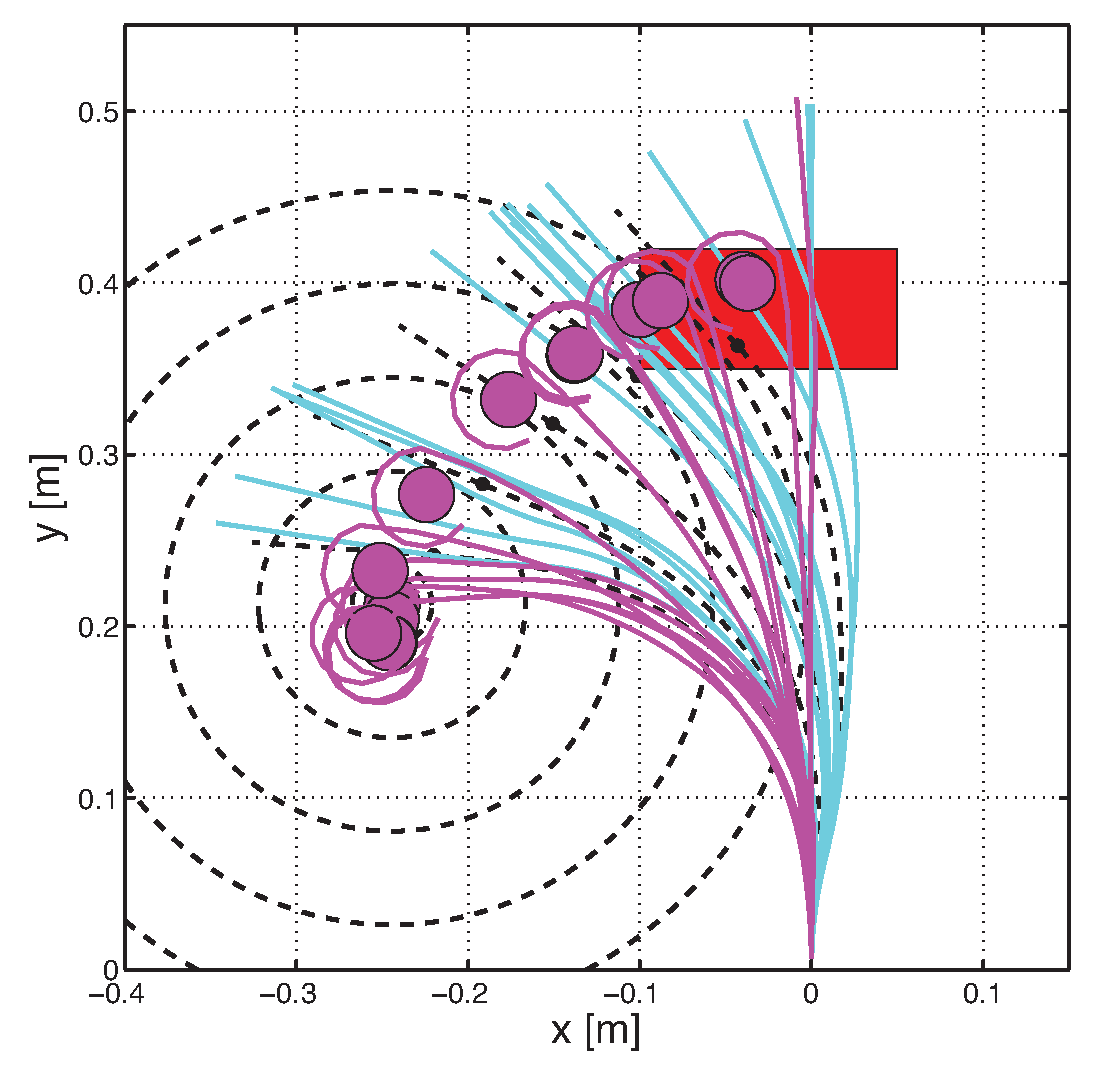
\includegraphics[width=0.375\textwidth]{Figures/experimental_results/oneTrialVsTime.eps}
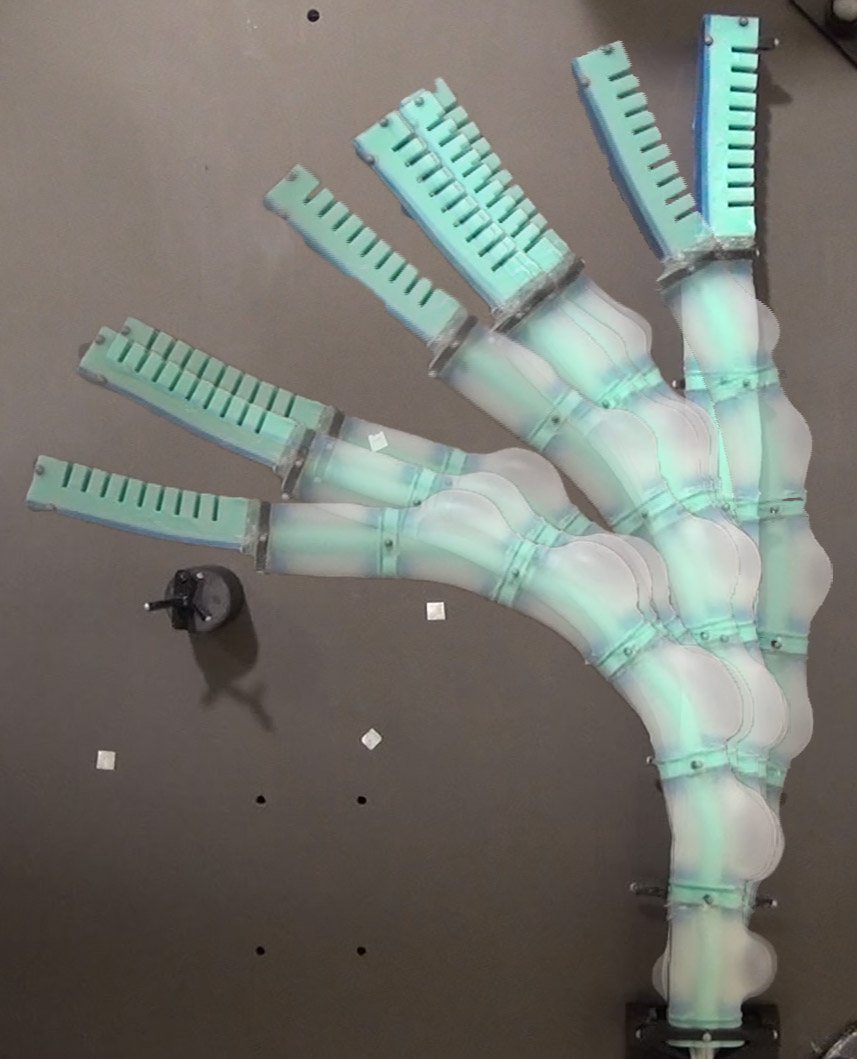
\includegraphics[width=0.30\textwidth]{figures/experimental_results/exp5a-4_sweep_to_object.jpg}
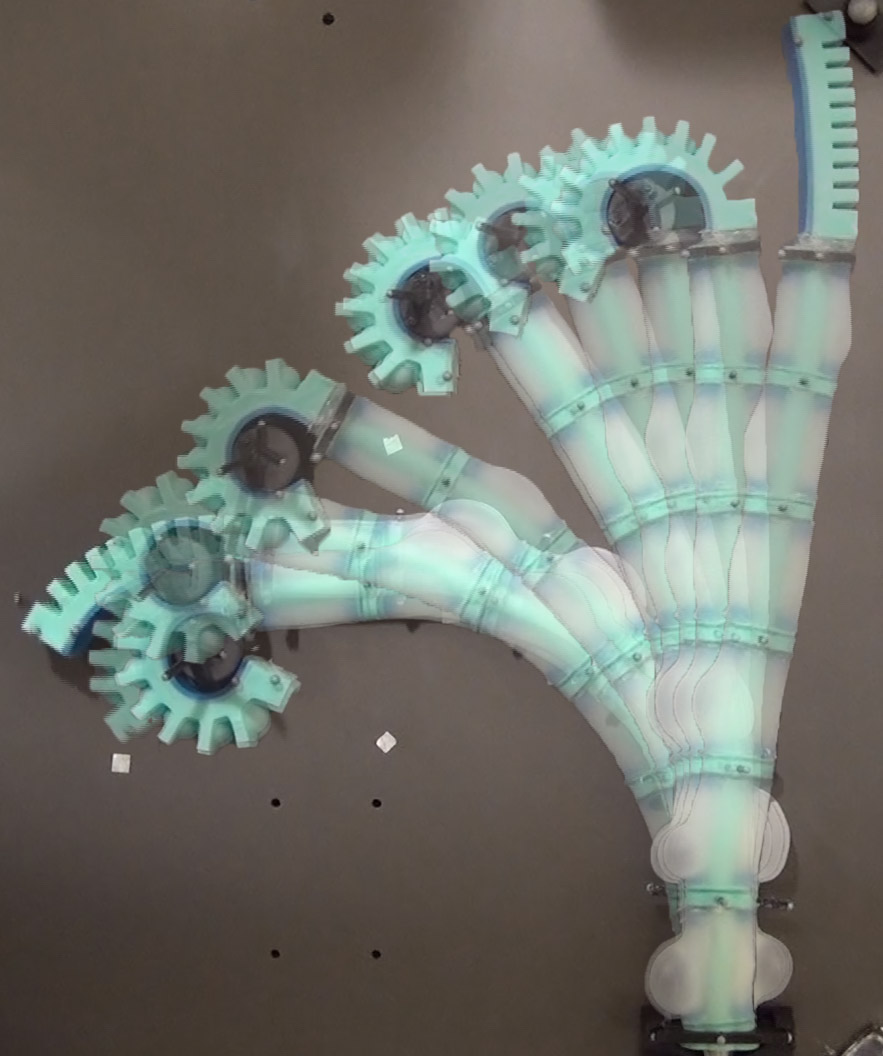
\includegraphics[width=0.31\textwidth]{figures/experimental_results/exp5a-4_sweep_to_bin.jpg}
  \caption{Left: A time series representation of an experimental grasp-and-place trial for an object located at point E (Figure~\ref{fig:allTestsOverlaid}). Here, the locally optimal planned manipulator configurations as well as planned sequential approach circles are shown as black dotted curves. The arm and gripper are shown in their experimentally determined configuration representations at 1 second intervals. The cyan configurations represent the manipulator prior to grasping the object, that is moving from its initial configuration to the object's location. \rkk{Depending on where the object is placed, the manipulator takes between 17-35\unit{s} to approach it.} After grasping the object, the magenta configurations represent the manipulator moving from the object's location back to the bin location shown in red. \rkk{This task of moving back to the bin takes between 10-20\unit{s}.} Right: Overlaid photographs of the manipulator moving from its initial pose to the object and from the object to the release location, respectively.}
\label{fig:oneTrialVsTime}
\end{centering}
\end{figure*}

\rkk{The experiments were performed for picking up objects on the left quadrant of the manipulator.
Grasping objects on both sides of the manipulator could be achieved in various ways including 
\begin{enumerate}
\item replacing the large gripper at the end of the arm with two smaller grippers next to each other, 
\item mounting roller supports on the top face of the manipulator and then rotating the manipulator at its root by $180^{\circ}$,
\item increasing the reachable workspace through starting the soft arm at an extreme curvature configuration within the right quadrant.  
\end{enumerate}
}